\documentclass[border=10pt]{standalone}
\usepackage[svgnames]{xcolor}
\usepackage{amsmath}
\usepackage{pgfplots}
\pgfplotsset{compat=newest}
\usepackage[sfdefault]{FiraSans}
\usepackage{FiraMono}
\renewcommand*\familydefault{\sfdefault}
\begin{document}
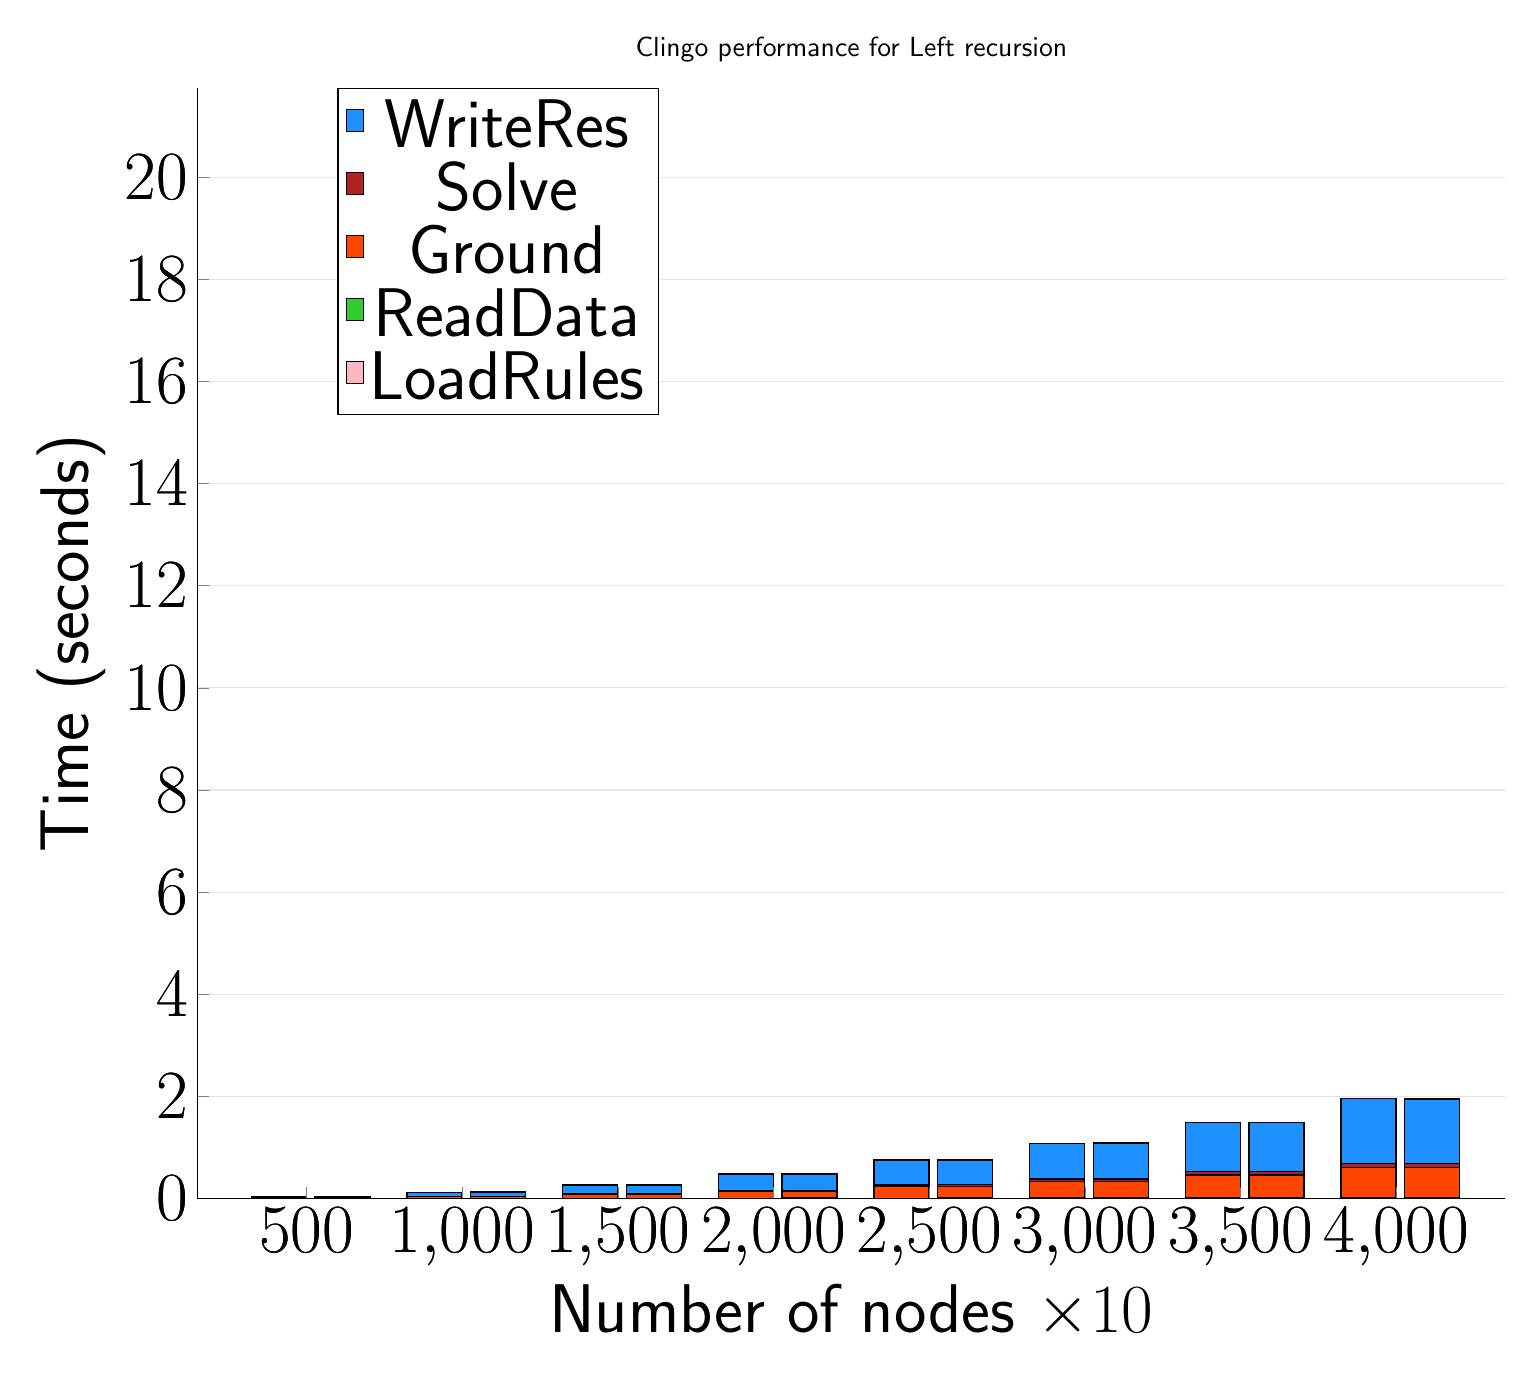
\begin{tikzpicture}
	\begin{axis}[
			ybar stacked,
			title={Clingo performance for Left recursion},
			bar shift=-10pt,
			width=1.5\textwidth,
			bar width=0.7cm,
			ymajorgrids, tick align=inside,
			major grid style={draw=gray!20},
			xtick=data,
			ymin=0, ymax=21.74900002479553,
			axis x line*=bottom,
			axis y line*=left,
			enlarge x limits=0.1,
			legend style={
					at={(0.23, 1)},
					anchor=north,
					legend columns=1,
					font=\Huge,
				},
			ylabel={Time (seconds)},
			xlabel={Number of nodes $\times 10$},
			label style={font=\Huge},
			tick label style={font=\Huge},
		]
		\addlegendimage{fill=DodgerBlue, draw=black, line width=0.2pt}
		\addlegendentry{WriteRes}
		\addlegendimage{fill=FireBrick, draw=black, line width=0.2pt}
		\addlegendentry{Solve}
		\addlegendimage{fill=OrangeRed, draw=black, line width=0.2pt}
		\addlegendentry{Ground}
		\addlegendimage{fill=LimeGreen, draw=black, line width=0.2pt}
		\addlegendentry{ReadData}
		\addlegendimage{fill=LightPink, draw=black, line width=0.2pt}
		\addlegendentry{LoadRules}
		\addplot +[fill=LightPink, draw=black, line width=0.5pt] coordinates {
				(500, 0.0)
				(1000, 0.0)
				(1500, 0.0)
				(2000, 0.0)
				(2500, 0.0)
				(3000, 0.0)
				(3500, 0.0)
				(4000, 0.0)
			};
		\addplot +[fill=LimeGreen, draw=black, line width=0.5pt] coordinates {
				(500, 0.0009999990463256836)
				(1000, 0.0009999990463256836)
				(1500, 0.005999994277954101)
				(2000, 0.004999995231628418)
				(2500, 0.004999995231628418)
				(3000, 0.009000015258789063)
				(3500, 0.010000014305114746)
				(4000, 0.009999990463256836)
			};
		\addplot +[fill=OrangeRed, draw=black, line width=0.5pt] coordinates {
				(500, 0.008999991416931152)
				(1000, 0.03700001239776611)
				(1500, 0.07799999713897705)
				(2000, 0.14000003337860106)
				(2500, 0.23000001907348633)
				(3000, 0.32799997329711916)
				(3500, 0.45299997329711916)
				(4000, 0.6009999990463257)
			};
		\addplot +[fill=FireBrick, draw=black, line width=0.5pt] coordinates {
				(500, 0.0009999990463256836)
				(1000, 0.0019999980926513673)
				(1500, 0.01100006103515625)
				(2000, 0.018999981880187988)
				(2500, 0.02999999523162842)
				(3000, 0.04600002765655518)
				(3500, 0.06500000953674316)
				(4000, 0.07899999618530273)
			};
		\addplot +[fill=DodgerBlue, draw=black, line width=0.5pt] coordinates {
				(500, 0.02000002861022949)
				(1000, 0.0820000171661377)
				(1500, 0.17399992942810058)
				(2000, 0.31700003147125244)
				(2500, 0.48900001049041747)
				(3000, 0.6979999542236328)
				(3500, 0.9609999656677246)
				(4000, 1.266000008583069)
			};
	\end{axis}
	\begin{axis}[
			ybar stacked,
			bar shift=13pt,
			width=1.5\textwidth,
			bar width=0.7cm,
			ymajorgrids, tick align=inside,
			major grid style={draw=none},
			xtick=data,
			ymin=0, ymax=21.74900002479553,
			axis x line*=none,
			axis y line*=none,
			enlarge x limits=0.1,
			label style={font=\Huge},
			tick label style={font=\Huge},
		]
		\addplot +[fill=LightPink, draw=black, line width=0.5pt] coordinates {
				(500, 0.0)
				(1000, 0.0)
				(1500, 0.0)
				(2000, 0.0)
				(2500, 0.0)
				(3000, 0.0)
				(3500, 0.0)
				(4000, 0.0)
			};
		\addplot +[fill=LimeGreen, draw=black, line width=0.5pt] coordinates {
				(500, 0.0)
				(1000, 0.0009999999999999998)
				(1500, 0.0)
				(2000, 0.009999999999999997)
				(2500, 0.009999999999999997)
				(3000, 0.009999999999999997)
				(3500, 0.009999999999999997)
				(4000, 0.009999999999999997)
			};
		\addplot +[fill=OrangeRed, draw=black, line width=0.5pt] coordinates {
				(500, 0.009999999999999997)
				(1000, 0.038999999999999986)
				(1500, 0.07999999999999999)
				(2000, 0.13199999999999998)
				(2500, 0.229)
				(3000, 0.33)
				(3500, 0.45200000000000007)
				(4000, 0.602)
			};
		\addplot +[fill=FireBrick, draw=black, line width=0.5pt] coordinates {
				(500, 0.0)
				(1000, 0.0010000000000000009)
				(1500, 0.009999999999999995)
				(2000, 0.01899999999999999)
				(2500, 0.03100000000000002)
				(3000, 0.04100000000000003)
				(3500, 0.06500000000000004)
				(4000, 0.07699999999999999)
			};
		\addplot +[fill=DodgerBlue, draw=black, line width=0.5pt] coordinates {
				(500, 0.020000000000000007)
				(1000, 0.08399999999999999)
				(1500, 0.17799999999999996)
				(2000, 0.32100000000000006)
				(2500, 0.48200000000000004)
				(3000, 0.7049999999999998)
				(3500, 0.9570000000000002)
				(4000, 1.261)
			};
	\end{axis}
\end{tikzpicture}

\end{document}
